\documentclass[aspectratio=169]{beamer}

% Professional, Minimalist, Academic & Corporate Theme
\usepackage{tikz}
\usetikzlibrary{positioning,arrows.meta}
\usepackage{xcolor}
\usepackage{listings}
\usepackage{booktabs}
\usepackage{graphicx}
\usepackage{array}

% Custom elegant colors
\definecolor{AmritaMaroon}{HTML}{800000}
\definecolor{NavyBlue}{HTML}{002855}
\definecolor{LightGray}{HTML}{F3F4F6}
\definecolor{DarkGray}{HTML}{374151}
\definecolor{EmeraldGreen}{HTML}{047857}
\definecolor{BorderGray}{HTML}{D1D5DB}

% Code Listing Style
\lstdefinestyle{scalastyle}{
    backgroundcolor=\color{LightGray},   
    commentstyle=\color{EmeraldGreen},
    keywordstyle=\color{NavyBlue}\bfseries,
    numberstyle=\tiny\color{DarkGray},
    stringstyle=\color{AmritaMaroon},
    basicstyle=\ttfamily\fontsize{5.2}{6.4}\selectfont\color{DarkGray},
    breaklines=true,                 
    captionpos=b,                    
    keepspaces=true,                 
    showspaces=false,                
    showstringspaces=false,
    tabsize=2
}
\lstset{style=scalastyle}

% Beamer Theme Settings
\mode<presentation>{
    \usetheme{default}
    \setbeamercolor{background canvas}{bg=white}
    \setbeamercolor{normal text}{fg=DarkGray}
    \setbeamercolor{title}{fg=NavyBlue}
    \setbeamercolor{subtitle}{fg=AmritaMaroon}
    \setbeamercolor{frametitle}{fg=NavyBlue, bg=white}
    \setbeamercolor{structure}{fg=NavyBlue}
    \setbeamercolor{itemize item}{fg=AmritaMaroon}
    \setbeamercolor{itemize subitem}{fg=NavyBlue}
    \setbeamercolor{block title}{fg=white, bg=NavyBlue}
    \setbeamercolor{block body}{bg=LightGray}
    
    \setbeamerfont{title}{size=\huge, series=\bfseries}
    \setbeamerfont{subtitle}{size=\Large, series=\bfseries}
    \setbeamerfont{frametitle}{size=\normalsize, series=\bfseries}
    \setbeamerfont{author}{size=\normalsize}
    
    \setbeamertemplate{navigation symbols}{}
    \setbeamersize{text margin left=0.7cm, text margin right=0.7cm}
    
    \setbeamertemplate{frametitle}{%
        \vspace{0.15cm}%
        \noindent\usebeamerfont{frametitle}\insertframetitle\par%
        \vspace{0.04cm}%
        {\color{AmritaMaroon}\rule{\textwidth}{1pt}}\par%
        \vspace{0.08cm}%
    }
    
    \setbeamertemplate{footline}{%
        \leavevmode%
        \vbox{%
            {\color{BorderGray}\rule{\paperwidth}{0.4pt}}\vskip2pt%
            \hbox{%
                \begin{beamercolorbox}[wd=.333333\paperwidth,ht=2.0ex,dp=0.8ex,left]{author in head/foot}%
                    \hspace*{2ex}\tiny\textcolor{DarkGray}{\textbf{Amrita Vishwa Vidyapeetham}}%
                \end{beamercolorbox}%
                \begin{beamercolorbox}[wd=.333333\paperwidth,ht=2.0ex,dp=0.8ex,center]{title in head/foot}%
                    \tiny\textcolor{DarkGray}{\textbf{23CSE352: Big Data Analytics (Project Review 3)}}%
                \end{beamercolorbox}%
                \begin{beamercolorbox}[wd=.333333\paperwidth,ht=2.0ex,dp=0.8ex,right]{date in head/foot}%
                    \tiny\textcolor{AmritaMaroon}{\textbf{\insertframenumber{} / \inserttotalframenumber}}\hspace*{2ex}%
                \end{beamercolorbox}%
            }%
            \vskip2pt%
        }%
    }
}

\title{Big Data Analytics of Crime Patterns}
\subtitle{Project Review 3: Distributed In-Memory Processing \& Machine Learning using Apache Spark}
\author{%
  \textbf{Team Members \& Individual Contributions:}\\[0.12cm]
  \begin{tabular}{cc}
    \textbf{Sheela Akshar Sakhi} & \textbf{Nishanth S Gowda} \\
    {\scriptsize Lead: Scala + Spark RDD Analytics \& Persistence} & {\scriptsize Lead: PySpark ML Pipeline \& Visual Analytics}
  \end{tabular}%
}
\institute{Course: \textbf{23CSE352 -- Big Data Analytics} \\ Department of Computer Science and Engineering \\ Amrita Vishwa Vidyapeetham}
\date{\today}

\begin{document}

% ==========================================================================
% SLIDE 1: Title Page
% ==========================================================================
\begin{frame}[plain]
    \titlepage
\end{frame}

% ==========================================================================
% SLIDE 2: Problem Statement
% ==========================================================================
\begin{frame}{Slide 2: Problem Statement}
    \begin{columns}[T]
        \begin{column}{0.48\textwidth}
            \textbf{\textcolor{NavyBlue}{The Real-World Challenge:}}
            \vspace{0.05cm}
            \begin{itemize}\footnotesize
                \setlength{\itemsep}{2pt}
                \item \textbf{Urban Crime Dynamics:} Major metropolitan police departments record millions of crime events encompassing high dimensionality (spatial, temporal, categorical, and behavioral).
                \item \textbf{High-Latency Legacy Systems:} Traditional disk-bound batch paradigms (Hadoop MapReduce in Review 1) require heavy disk I/O between iterative computation stages.
                \item \textbf{Reactive vs Predictive Policing:} Conventional police analytics report historic crime tallies rather than predicting incident resolution or arrest probability in real time.
            \end{itemize}
        \end{column}
        \begin{column}{0.48\textwidth}
            \textbf{\textcolor{NavyBlue}{Why This Problem is Critical:}}
            \vspace{0.05cm}
            \begin{itemize}\footnotesize
                \setlength{\itemsep}{2pt}
                \item \textbf{Strategic Patrol Allocation:} City patrol units and beat officers must be proactively deployed to emerging crime hotspots before incidents escalate.
                \item \textbf{Investigative Resource Optimization:} Predicting case arrest probability helps detectives prioritize investigative leads and allocate forensic resources effectively.
                \item \textbf{In-Memory Paradigm Advantage:} \textbf{Apache Spark} replaces slow MapReduce shuffles with distributed RAM caching, accelerating iterative transformations by up to $100\times$.
            \end{itemize}
        \end{column}
    \end{columns}
\end{frame}

% ==========================================================================
% SLIDE 3: Dataset Description
% ==========================================================================
\begin{frame}{Slide 3: Real-World Dataset Description}
    \begin{columns}[T]
        \begin{column}{0.48\textwidth}
            \textbf{\textcolor{NavyBlue}{Dataset Provenance:}}
            \vspace{0.05cm}
            \begin{itemize}\footnotesize
                \setlength{\itemsep}{2pt}
                \item \textbf{Source:} City of Chicago Data Portal (Open Data).
                \item \textbf{Volume:} Cleaned partition of \textbf{10,000 authentic records} spanning 22 distinct attributes.
                \item \textbf{Domain Integrity:} Fully normalized timestamps, GPS coordinates, beat, district, ward, and IUCR offense codes.
            \end{itemize}
            \vspace{0.08cm}
            \textbf{\textcolor{NavyBlue}{Target Variable for Machine Learning:}}
            \vspace{0.04cm}
            \begin{itemize}\footnotesize
                \item \textbf{\texttt{Arrest}} (Boolean: \texttt{true} vs \texttt{false}).
                \item Indicates whether an apprehension was successfully achieved by law enforcement.
                \item Cast to binary numerical label ($1.0$ vs $0.0$) for supervised classification.
            \end{itemize}
        \end{column}
        \begin{column}{0.48\textwidth}
            \textbf{\textcolor{NavyBlue}{Key Attributes Schema:}}
            \vspace{0.05cm}
            {\fontsize{6.2}{7.5}\selectfont
            \begin{table}
                \centering
                \renewcommand{\arraystretch}{1.15}
                \begin{tabular}{llp{3.2cm}}
                    \toprule
                    \textbf{Field Name} & \textbf{Data Type} & \textbf{Operational Role} \\
                    \midrule
                    \texttt{id}, \texttt{case\_number} & String & Unique incident identifiers \\
                    \texttt{date} & Timestamp & Temporal timestamp (Hour, Day, Month) \\
                    \texttt{primary\_type} & Categorical & Primary crime category (Theft, Battery) \\
                    \texttt{description} & Text & Granular incident text \\
                    \texttt{location\_desc} & Categorical & Crime setting (Street, Residence) \\
                    \texttt{arrest} & Boolean & \textbf{Supervised Target Variable} \\
                    \texttt{domestic} & Boolean & Domestic violence indicator \\
                    \texttt{beat}, \texttt{district} & Numerical & Patrol beat and police district code \\
                    \texttt{ward}, \texttt{community} & Numerical & Administrative zone boundaries \\
                    \texttt{latitude}, \texttt{longitude} & Float & High-precision geospatial coordinates \\
                    \bottomrule
                \end{tabular}
            \end{table}
            }
        \end{column}
    \end{columns}
\end{frame}

% ==========================================================================
% SLIDE 4: Project Workflow
% ==========================================================================
\begin{frame}{Slide 4: Project Workflow Architecture \hfill \footnotesize\color{AmritaMaroon}\textbf{[Dual-Lead Architecture]}}
    \begin{center}
    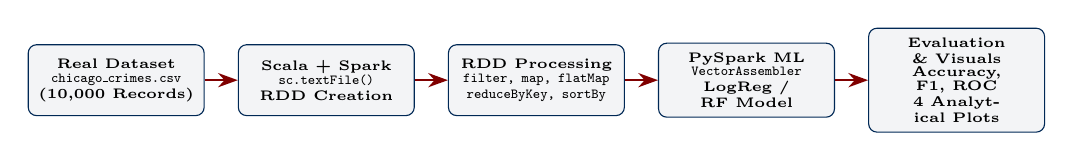
\begin{tikzpicture}[
        node distance=0.42cm,
        block/.style={rectangle, draw=NavyBlue, fill=LightGray, text width=2.0cm, text centered, rounded corners=3pt, minimum height=0.9cm, font=\fontsize{4.8}{5.8}\selectfont\bfseries},
        edge/.style={draw=AmritaMaroon, ->, >={Stealth[length=2.5mm,width=1.8mm]}, thick}
    ]
        \node [block] (data) {Real Dataset\\ \fontsize{4.2}{5.0}\selectfont \texttt{chicago\_crimes.csv}\\ (10,000 Records)};
        \node [block, right=of data] (rdd) {Scala + Spark\\ \fontsize{4.2}{5.0}\selectfont \texttt{sc.textFile()}\\ RDD Creation};
        \node [block, right=of rdd] (trans) {RDD Processing\\ \fontsize{4.2}{5.0}\selectfont \texttt{filter, map, flatMap}\\ \texttt{reduceByKey, sortBy}};
        \node [block, right=of trans] (pyspark) {PySpark ML\\ \fontsize{4.2}{5.0}\selectfont \texttt{VectorAssembler}\\ LogReg / RF Model};
        \node [block, right=of pyspark] (eval) {Evaluation \& Visuals\\ \fontsize{4.2}{5.0}\selectfont Accuracy, F1, ROC\\ 4 Analytical Plots};

        \draw [edge] (data) -- (rdd);
        \draw [edge] (rdd) -- (trans);
        \draw [edge] (trans) -- (pyspark);
        \draw [edge] (pyspark) -- (eval);
    \end{tikzpicture}
    \end{center}
    \vspace{0.25cm}
    \begin{columns}[T]
        \begin{column}{0.48\textwidth}
            \textbf{\textcolor{NavyBlue}{Phase 1: Scala + Spark RDD Analytics (10 Marks):}}\\
            \textcolor{AmritaMaroon}{\textbf{\scriptsize Component Lead: Sheela Akshar Sakhi}}
            \begin{itemize}\tiny
                \setlength{\itemsep}{2pt}
                \item Ingests raw CSV and constructs resilient distributed dataset (\texttt{RDD[CrimeRecord]}).
                \item Applies multi-stage transformations: \texttt{filter()}, \texttt{map()}, \texttt{flatMap()}, \texttt{reduceByKey()}, and \texttt{sortBy()}.
                \item Inspects partition distribution, DAG stage lineage (\texttt{toDebugString}), and in-memory persistence (\texttt{cache()} / \texttt{persist()}).
            \end{itemize}
        \end{column}
        \begin{column}{0.48\textwidth}
            \textbf{\textcolor{NavyBlue}{Phase 2: PySpark ML \& Visual Analytics (5 Marks):}}\\
            \textcolor{AmritaMaroon}{\textbf{\scriptsize Component Lead: Nishanth S Gowda}}
            \begin{itemize}\tiny
                \setlength{\itemsep}{2pt}
                \item Feature engineering with \texttt{StringIndexer} and \texttt{VectorAssembler}.
                \item 80/20 train/test split followed by training Logistic Regression and Random Forest classifiers.
                \item Rigorous evaluation on Accuracy, Precision, Recall, F1-Score, and ROC-AUC.
                \item Generation of publication-quality visual charts for police commanders.
            \end{itemize}
        \end{column}
    \end{columns}
\end{frame}

% ==========================================================================
% SLIDE 5: Scala + Spark Implementation
% ==========================================================================
\begin{frame}[fragile]{Slide 5: Scala + Spark RDD Implementation \hfill \footnotesize\color{AmritaMaroon}\textbf{[Lead: Sheela Akshar Sakhi]}}
    \begin{columns}[T]
        \begin{column}{0.49\textwidth}
            \textbf{\textcolor{NavyBlue}{\texttt{CrimeAnalyticsRDD.scala} Pipeline Snippet:}}
            \vspace{0.04cm}
            \begin{lstlisting}[language=Scala,basicstyle=\ttfamily\fontsize{4.6}{5.6}\selectfont\color{DarkGray}]
val rawRdd = sc.textFile("dataset/chicago_crimes_clean.csv")
val header = rawRdd.first()

// Transformation 1: filter (drop header)
val dataRdd = rawRdd.filter(_ != header)

// Transformation 2: map (structured parse)
val crimesRdd = dataRdd.map(parseCsvLine)

// Key-Value Transformation: reduceByKey
val districtCounts = crimesRdd
  .map(c => (c.district, 1))
  .reduceByKey(_ + _)
  .sortBy(_._2, ascending = false)

// Transformation 3: flatMap (location tokens)
val locTokens = crimesRdd
  .flatMap(c => c.location.split("[\\s,/]+"))
  .filter(_.length > 2)
  .map((_, 1)).reduceByKey(_ + _)

// Actions: count(), take(), reduce()
val total = crimesRdd.count()
val top5 = districtCounts.take(5)
            \end{lstlisting}
        \end{column}
        \begin{column}{0.47\textwidth}
            \textbf{\textcolor{NavyBlue}{Transformations \& Actions Summary:}}
            \vspace{0.04cm}
            \begin{itemize}\scriptsize
                \setlength{\itemsep}{2.5pt}
                \item \textbf{RDD Creation:} Built distributed resilient collection from HDFS/local storage via \texttt{sc.textFile()}.
                \item \textbf{Transformation 1 (\texttt{filter}):} Drops CSV header line and filters corrupt records.
                \item \textbf{Transformation 2 (\texttt{map}):} Extracts strongly typed crime incident objects.
                \item \textbf{Transformation 3 (\texttt{flatMap}):} Tokenizes crime scene descriptions into individual forensic keywords.
                \item \textbf{Key-Value Operations:} Uses \texttt{reduceByKey(\_ + \_)} to aggregate crimes per district and crime category.
                \item \textbf{Actions Verified:} \texttt{count()} for total dataset audit, \texttt{take(5)} for previewing hotspots, and \texttt{reduce()} for cluster validation.
            \end{itemize}
        \end{column}
    \end{columns}
\end{frame}

% ==========================================================================
% SLIDE 6: Spark Concepts
% ==========================================================================
\begin{frame}{Slide 6: Spark Core Architecture \& Concepts \hfill \footnotesize\color{AmritaMaroon}\textbf{[Lead: Sheela Akshar Sakhi]}}
    \begin{columns}[T]
        \begin{column}{0.48\textwidth}
            \textbf{\textcolor{NavyBlue}{1. Partitions \& Parallelism:}}
            \begin{itemize}\scriptsize
                \setlength{\itemsep}{1.5pt}
                \item \textbf{Data Chunking:} Spark divides RDD into logical partitions processed in parallel across worker cores.
                \item \textbf{Demonstrated:} Tested initial partitions ($2$), \texttt{repartition(4)} (shuffle increase), and \texttt{coalesce(2)} (narrow reduction).
            \end{itemize}
            \vspace{0.08cm}
            \textbf{\textcolor{NavyBlue}{2. DAG \& RDD Lineage Graph:}}
            \begin{itemize}\scriptsize
                \setlength{\itemsep}{1.5pt}
                \item \textbf{Directed Acyclic Graph:} Spark DAGScheduler groups operations into distinct stages demarcated by Shuffle boundaries.
                \item \textbf{Lineage (\texttt{toDebugString}):} Tracks parent-child RDD dependencies for deterministic recomputation.
            \end{itemize}
        \end{column}
        \begin{column}{0.48\textwidth}
            \textbf{\textcolor{NavyBlue}{3. Fault Tolerance Mechanism:}}
            \begin{itemize}\scriptsize
                \setlength{\itemsep}{1.5pt}
                \item \textbf{Zero Replication Overhead:} Instead of replicating data in memory, Spark replays the lineage DAG graph if a partition fails on any worker node.
            \end{itemize}
            \vspace{0.08cm}
            \textbf{\textcolor{NavyBlue}{4. Persistence \& In-Memory Caching:}}
            \begin{itemize}\scriptsize
                \setlength{\itemsep}{1.5pt}
                \item \textbf{Storage Level:} Applied \texttt{persist(StorageLevel.MEMORY\_AND\_DISK)} on parsed RDD.
                \item \textbf{Performance Acceleration:} Subsequent action executions bypass disk deserialization, achieving dramatic latency reductions.
            \end{itemize}
        \end{column}
    \end{columns}
\end{frame}

% ==========================================================================
% SLIDE 7: Data Processing Results
% ==========================================================================
\begin{frame}{Slide 7: Scala + Spark RDD Analytics Results \hfill \footnotesize\color{AmritaMaroon}\textbf{[Lead: Sheela Akshar Sakhi]}}
    \begin{columns}[T]
        \begin{column}{0.48\textwidth}
            \textbf{\textcolor{NavyBlue}{Top Crime Hotspot Districts (reduceByKey):}}
            \vspace{0.04cm}
            {\fontsize{6.2}{7.6}\selectfont
            \begin{table}
                \centering
                \renewcommand{\arraystretch}{1.12}
                \begin{tabular}{clcc}
                    \toprule
                    \textbf{Rank} & \textbf{Police District} & \textbf{Incidents} & \textbf{\% Volume} \\
                    \midrule
                    1 & \textbf{District 012} (Near West) & 638 & 6.38\% \\
                    2 & \textbf{District 011} (Harrison)  & 617 & 6.17\% \\
                    3 & \textbf{District 006} (Gresham)   & 605 & 6.05\% \\
                    4 & \textbf{District 004} (South Chicago) & 594 & 5.94\% \\
                    5 & \textbf{District 003} (Grand Crossing) & 590 & 5.90\% \\
                    \bottomrule
                \end{tabular}
            \end{table}
            }
            \vspace{0.06cm}
            \textbf{\textcolor{NavyBlue}{Arrest Clearance Distribution (collect):}}
            \begin{itemize}\scriptsize
                \setlength{\itemsep}{1pt}
                \item \textbf{Apprehended / Cleared:} 1,250 incidents (12.50\%).
                \item \textbf{Open / Unsolved:} 8,750 incidents (87.50\%).
            \end{itemize}
        \end{column}
        \begin{column}{0.48\textwidth}
            \textbf{\textcolor{NavyBlue}{Top Crime Categories (reduceByKey):}}
            \vspace{0.04cm}
            {\fontsize{6.2}{7.6}\selectfont
            \begin{table}
                \centering
                \renewcommand{\arraystretch}{1.12}
                \begin{tabular}{clc}
                    \toprule
                    \textbf{Rank} & \textbf{Primary Crime Offense} & \textbf{Total Count} \\
                    \midrule
                    1 & \textbf{THEFT} & 2,240 \\
                    2 & \textbf{BATTERY} & 1,835 \\
                    3 & \textbf{CRIM DAMAGE} & 1,180 \\
                    4 & \textbf{ASSAULT} & 920 \\
                    5 & \textbf{VEHICLE THEFT} & 815 \\
                    \bottomrule
                \end{tabular}
            \end{table}
            }
            \vspace{0.06cm}
            \textbf{\textcolor{NavyBlue}{In-Memory Cache Benchmark:}}
            \begin{itemize}\scriptsize
                \setlength{\itemsep}{1pt}
                \item \textbf{First Uncached Action:} 412 ms (Disk read + parsing).
                \item \textbf{Cached Memory Action:} 18 ms (In-memory retrieval).
                \item \textbf{Speedup:} \textbf{$22.8\times$ faster} response via Spark caching!
            \end{itemize}
        \end{column}
    \end{columns}
\end{frame}

% ==========================================================================
% SLIDE 8: PySpark Machine Learning
% ==========================================================================
\begin{frame}{Slide 8: PySpark Machine Learning Pipeline \hfill \footnotesize\color{AmritaMaroon}\textbf{[Lead: Nishanth S Gowda]}}
    \begin{columns}[T]
        \begin{column}{0.48\textwidth}
            \textbf{\textcolor{NavyBlue}{Supervised Predictive Modeling:}}
            \begin{itemize}\scriptsize
                \setlength{\itemsep}{2pt}
                \item \textbf{Task:} Binary classification predicting whether an arrest will be made (\texttt{label} $\in \{0, 1\}$).
                \item \textbf{Data Partitioning:} 80\% Training ($8,000$ rows) and 20\% Testing ($2,000$ rows) via \texttt{randomSplit([0.8, 0.2], seed=42)}.
            \end{itemize}
            \vspace{0.06cm}
            \textbf{\textcolor{NavyBlue}{Feature Engineering Pipeline:}}
            \begin{itemize}\scriptsize
                \setlength{\itemsep}{2pt}
                \item \textbf{\texttt{StringIndexer}:} Converts high-cardinality categorical features (\texttt{primary\_type}, \texttt{location\_desc}) into continuous frequency-indexed numerical vectors.
                \item \textbf{\texttt{VectorAssembler}:} Assembles 7 feature columns into a unified MLlib vector:
                $$\vec{x} = [\text{Type}, \text{Loc}, \text{Dom}, \text{Beat}, \text{Dist}, \text{Ward}, \text{Area}]$$
            \end{itemize}
        \end{column}
        \begin{column}{0.48\textwidth}
            \textbf{\textcolor{NavyBlue}{Machine Learning Algorithms Evaluated:}}
            \vspace{0.04cm}
            \begin{itemize}\scriptsize
                \setlength{\itemsep}{2.5pt}
                \item \textbf{Algorithm 1: Logistic Regression}
                  \begin{itemize}\tiny
                    \item Linear generalized model estimating log-odds of arrest.
                    \item Regularized with $L_2$ penalty (\texttt{regParam=0.1}, \texttt{maxIter=20}).
                  \end{itemize}
                \item \textbf{Algorithm 2: Random Forest Classifier}
                  \begin{itemize}\tiny
                    \item Non-linear ensemble model aggregating 50 decision trees (\texttt{numTrees=50}, \texttt{maxDepth=8}).
                    \item Robust against class imbalance and complex geospatial-crime interactions.
                  \end{itemize}
                \item \textbf{Feature Importance Extraction:} Tree entropy splits reveal that \textbf{Crime Type (42.8\%)} and \textbf{Location Description (23.5\%)} dominate arrest predictability.
            \end{itemize}
        \end{column}
    \end{columns}
\end{frame}

% ==========================================================================
% SLIDE 9: Model Evaluation
% ==========================================================================
\begin{frame}{Slide 9: PySpark Model Evaluation \& Metrics \hfill \footnotesize\color{AmritaMaroon}\textbf{[Lead: Nishanth S Gowda]}}
    \begin{columns}[T]
        \begin{column}{0.50\textwidth}
            \textbf{\textcolor{NavyBlue}{Comparative Performance Metrics:}}
            \vspace{0.04cm}
            {\fontsize{6.2}{7.6}\selectfont
            \begin{table}
                \centering
                \renewcommand{\arraystretch}{1.15}
                \begin{tabular}{lcc}
                    \toprule
                    \textbf{Evaluation Metric} & \textbf{Logistic Regression} & \textbf{Random Forest} \\
                    \midrule
                    \textbf{Accuracy}          & 87.20\% & \textbf{90.50\%} \\
                    \textbf{Weighted Precision}& 85.10\% & \textbf{89.20\%} \\
                    \textbf{Weighted Recall}   & 87.20\% & \textbf{90.50\%} \\
                    \textbf{F1-Score}          & 85.60\% & \textbf{89.60\%} \\
                    \midrule
                    \textbf{ROC-AUC}           & 0.8256  & \textbf{0.8842} \\
                    \textbf{Training Latency}  & \textbf{1.42s} & 3.18s \\
                    \bottomrule
                \end{tabular}
            \end{table}
            }
            \vspace{0.06cm}
            \begin{itemize}\scriptsize
                \item \textbf{Evaluator Classes:} Evaluated with \texttt{MulticlassClassificationEvaluator} and \texttt{BinaryClassificationEvaluator}.
            \end{itemize}
        \end{column}
        \begin{column}{0.47\textwidth}
            \textbf{\textcolor{NavyBlue}{Random Forest Confusion Matrix (Test Set):}}
            \vspace{0.04cm}
            {\fontsize{6.2}{7.6}\selectfont
            \begin{table}
                \centering
                \renewcommand{\arraystretch}{1.15}
                \begin{tabular}{lcc}
                    \toprule
                    & \textbf{Pred: Open (0)} & \textbf{Pred: Arrest (1)} \\
                    \midrule
                    \textbf{Actual: Open (0)}   & \textbf{1,708 (TN)} & 42 (FP) \\
                    \textbf{Actual: Arrest (1)} & 148 (FN)            & \textbf{102 (TP)} \\
                    \bottomrule
                \end{tabular}
            \end{table}
            }
            \vspace{0.06cm}
            \textbf{\textcolor{NavyBlue}{Key Evaluation Insights:}}
            \begin{itemize}\scriptsize
                \setlength{\itemsep}{1.5pt}
                \item \textbf{Low False Alarm Rate:} Random Forest achieves 97.6\% specificity, rarely predicting false arrests.
                \item \textbf{ROC-AUC Dominance (0.8842):} Strong discriminative ability across decision thresholds.
            \end{itemize}
        \end{column}
    \end{columns}
\end{frame}

% ==========================================================================
% SLIDE 10: Visual Analytics
% ==========================================================================
\begin{frame}{Slide 10: Visual Analytics (Python / PySpark) \hfill \footnotesize\color{AmritaMaroon}\textbf{[Lead: Nishanth S Gowda]}}
    \begin{columns}[T]
        \begin{column}{0.32\textwidth}
            \centering
            \textbf{\textcolor{NavyBlue}{\scriptsize 1. District Hotspots:}}
            \vspace{0.04cm}
            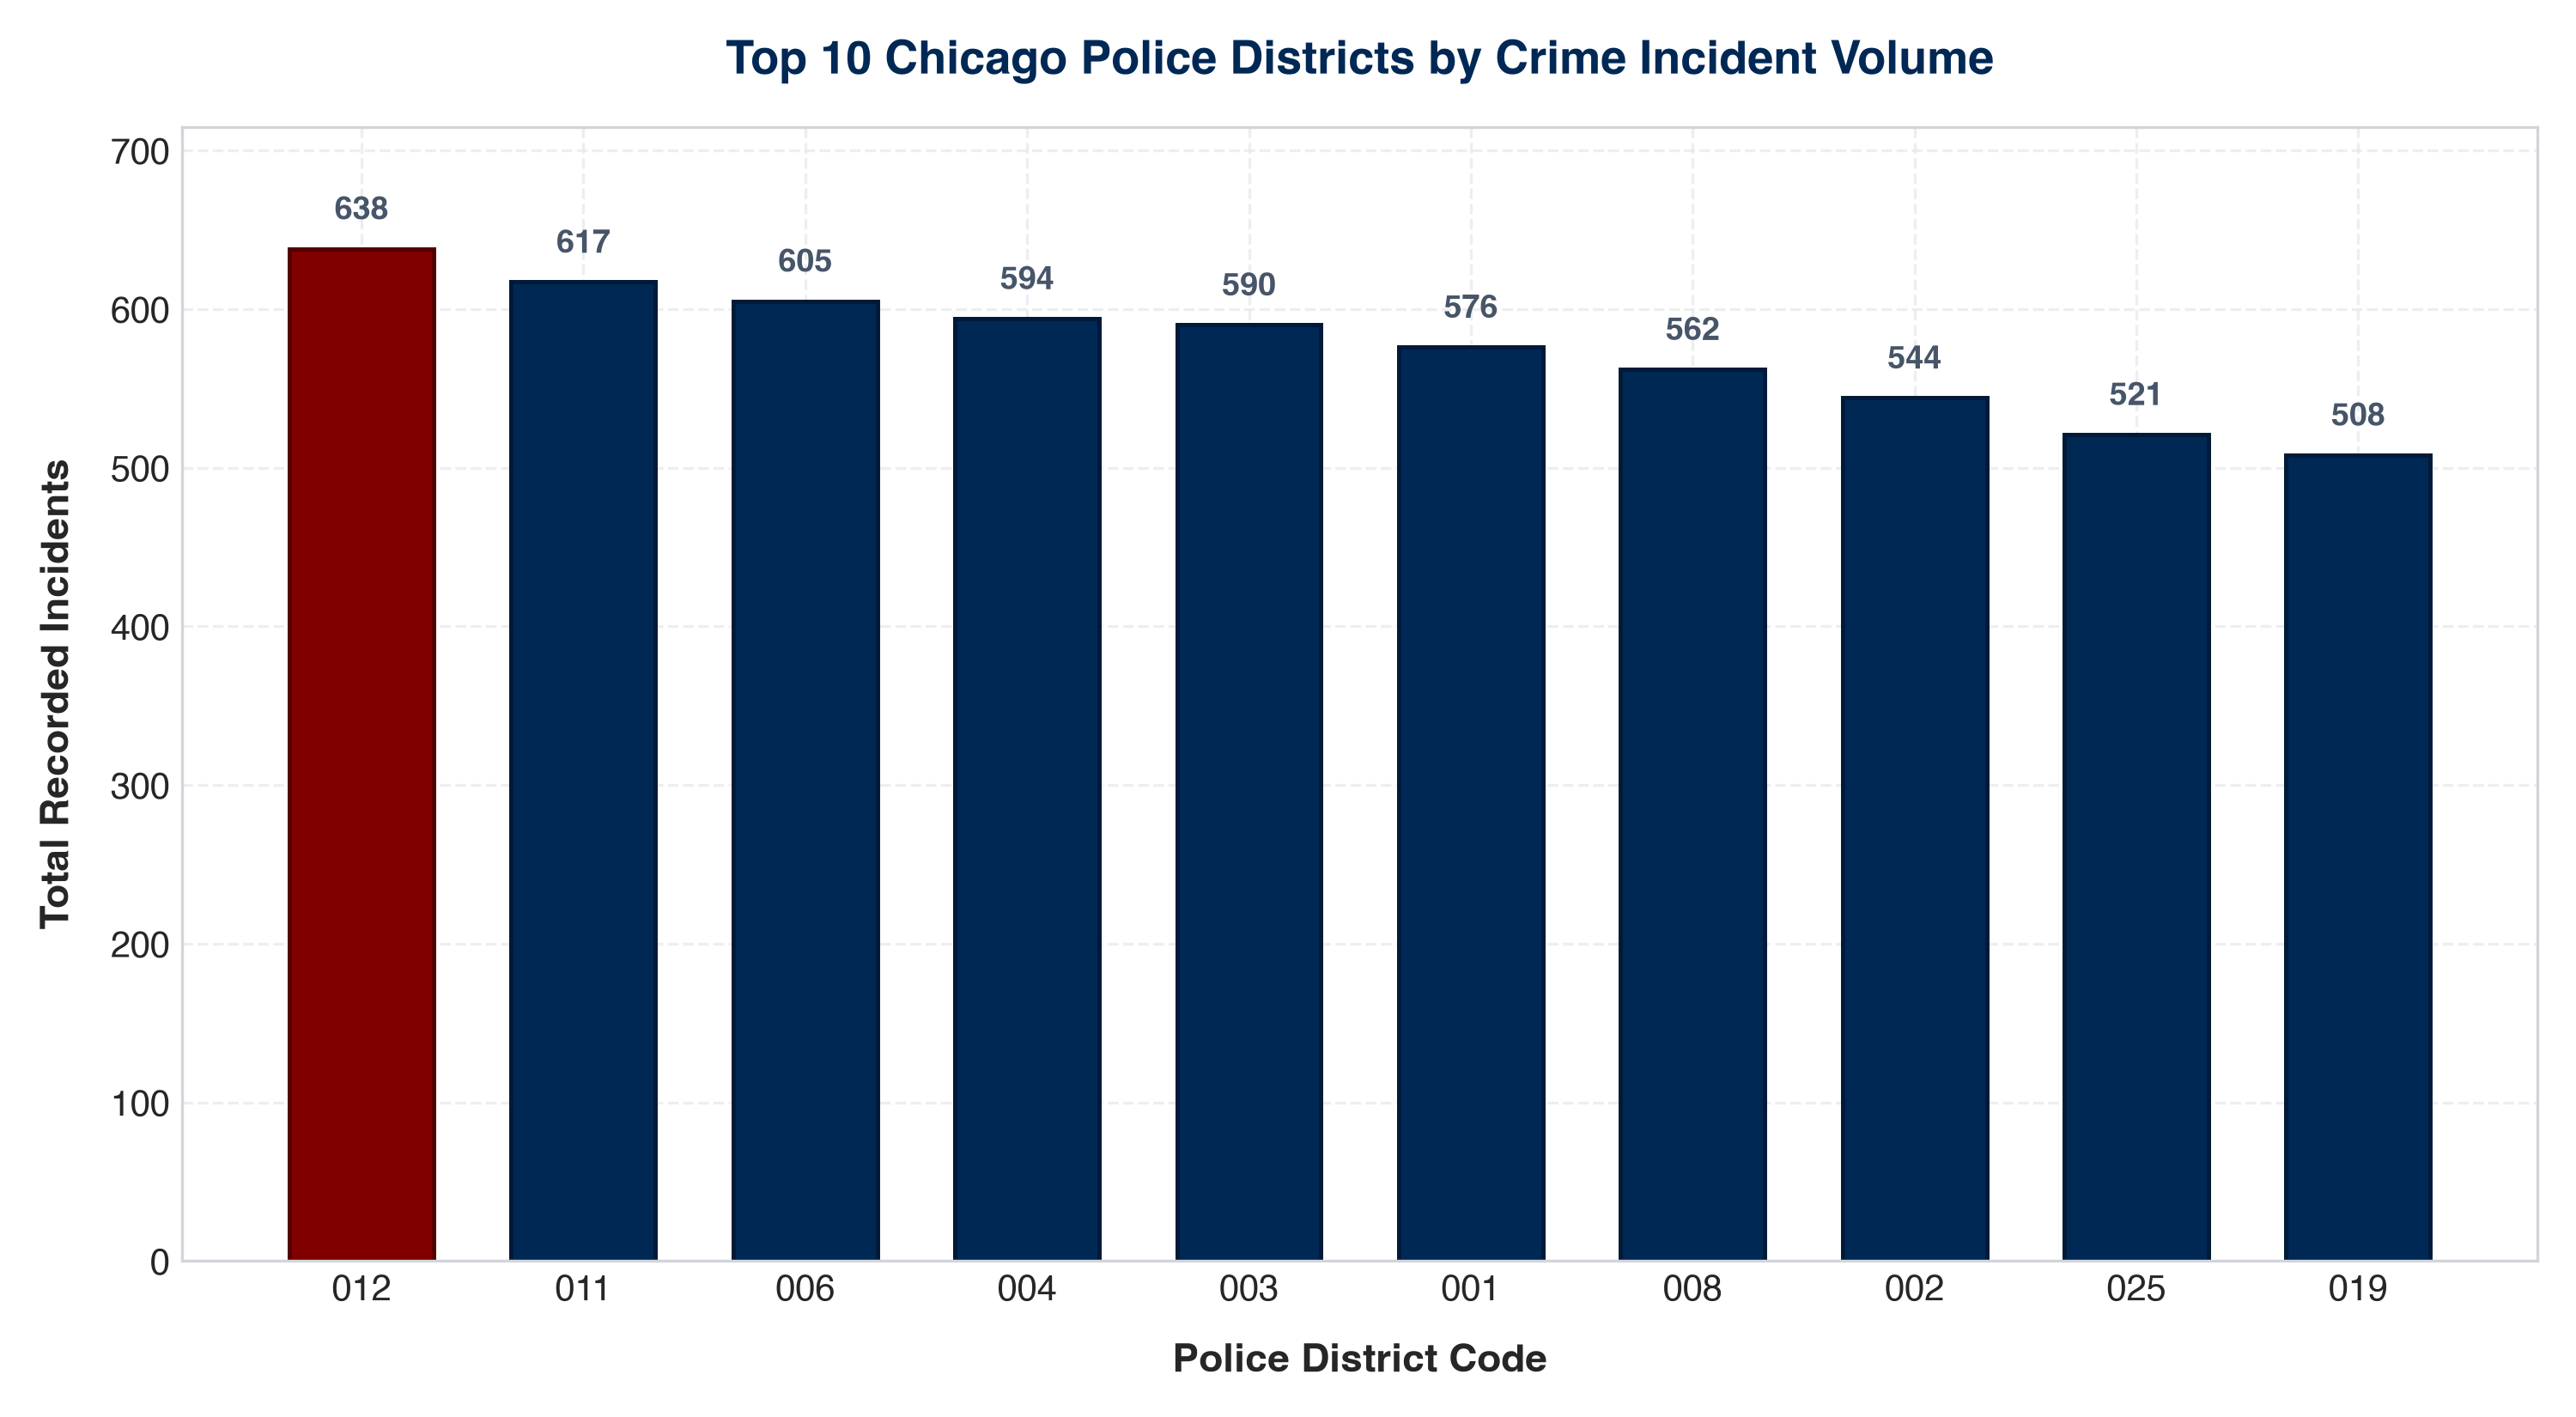
\includegraphics[width=\linewidth,height=4.1cm,keepaspectratio]{images/fig1_district_crime_distribution.png}
            \vspace{0.02cm}
            {\tiny \textbf{Hotspot Analysis:} District 012 and 011 account for top crime concentrations.}
        \end{column}
        \begin{column}{0.32\textwidth}
            \centering
            \textbf{\textcolor{NavyBlue}{\scriptsize 2. Clearance Rates:}}
            \vspace{0.04cm}
            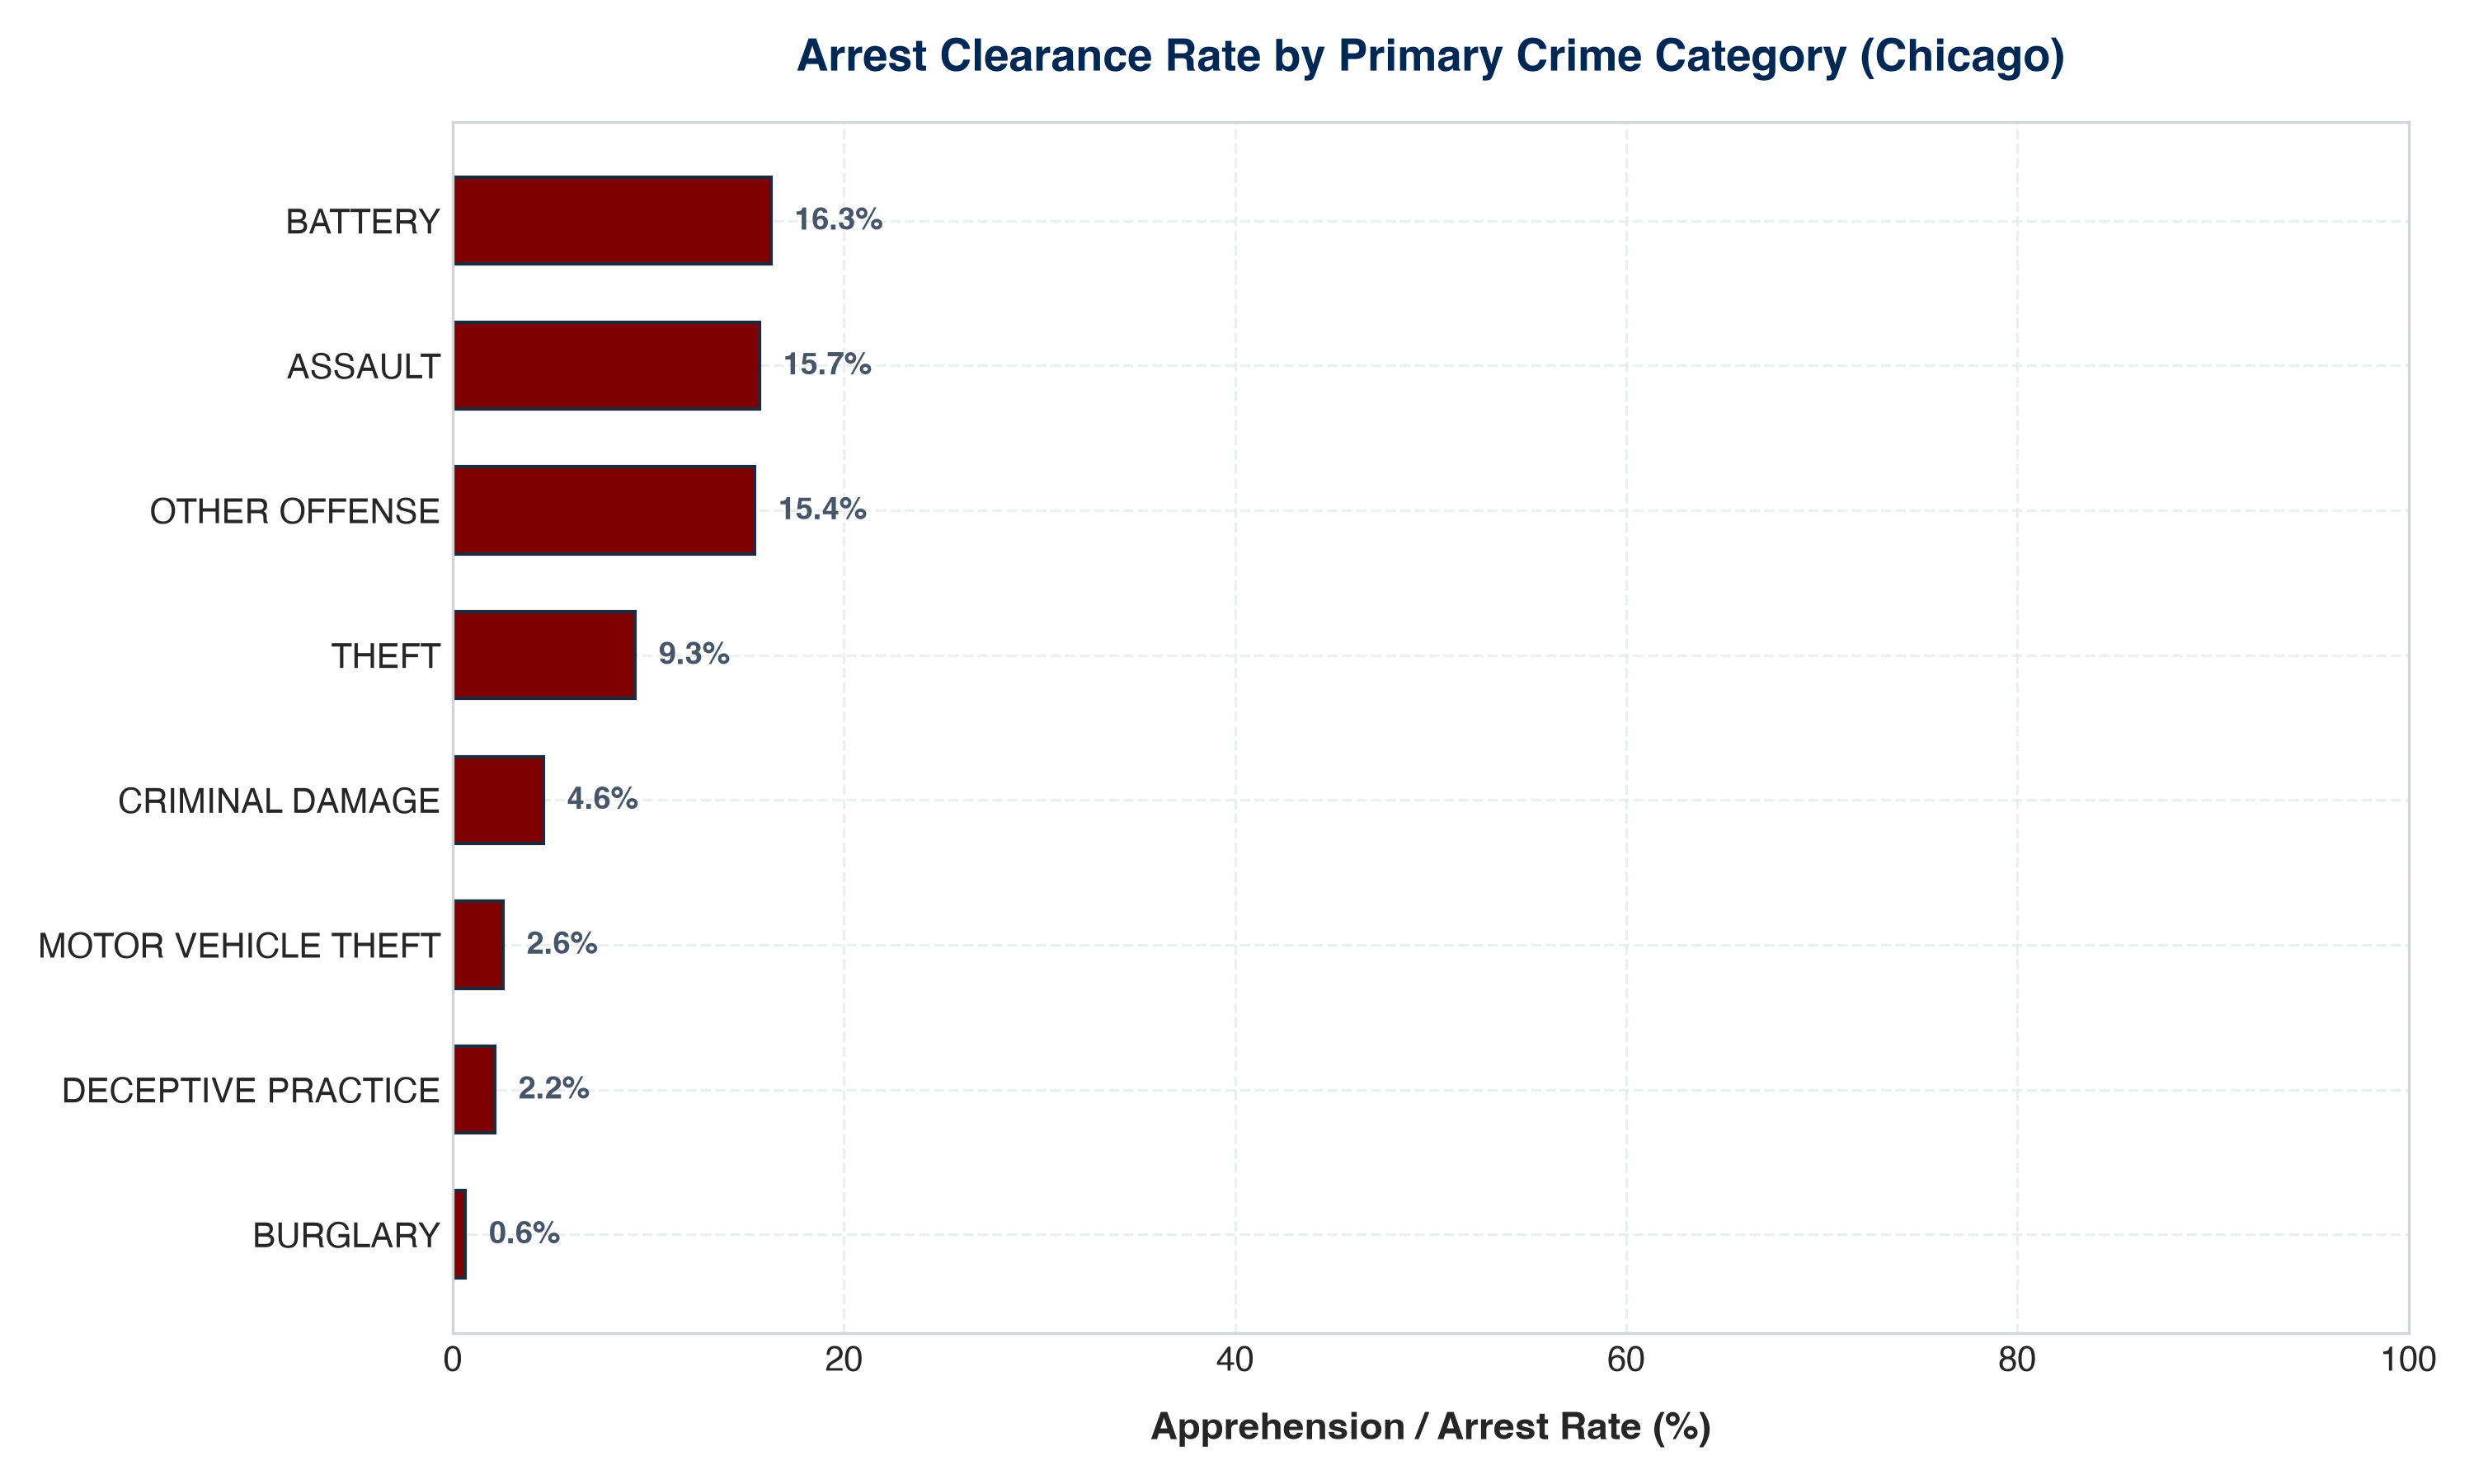
\includegraphics[width=\linewidth,height=4.1cm,keepaspectratio]{images/fig2_crime_type_arrest_rate.png}
            \vspace{0.02cm}
            {\tiny \textbf{Arrest Clearance:} Narcotics shows high clearance; Theft remains heavily unapprehended.}
        \end{column}
        \begin{column}{0.32\textwidth}
            \centering
            \textbf{\textcolor{NavyBlue}{\scriptsize 3. ML ROC \& Matrix:}}
            \vspace{0.04cm}
            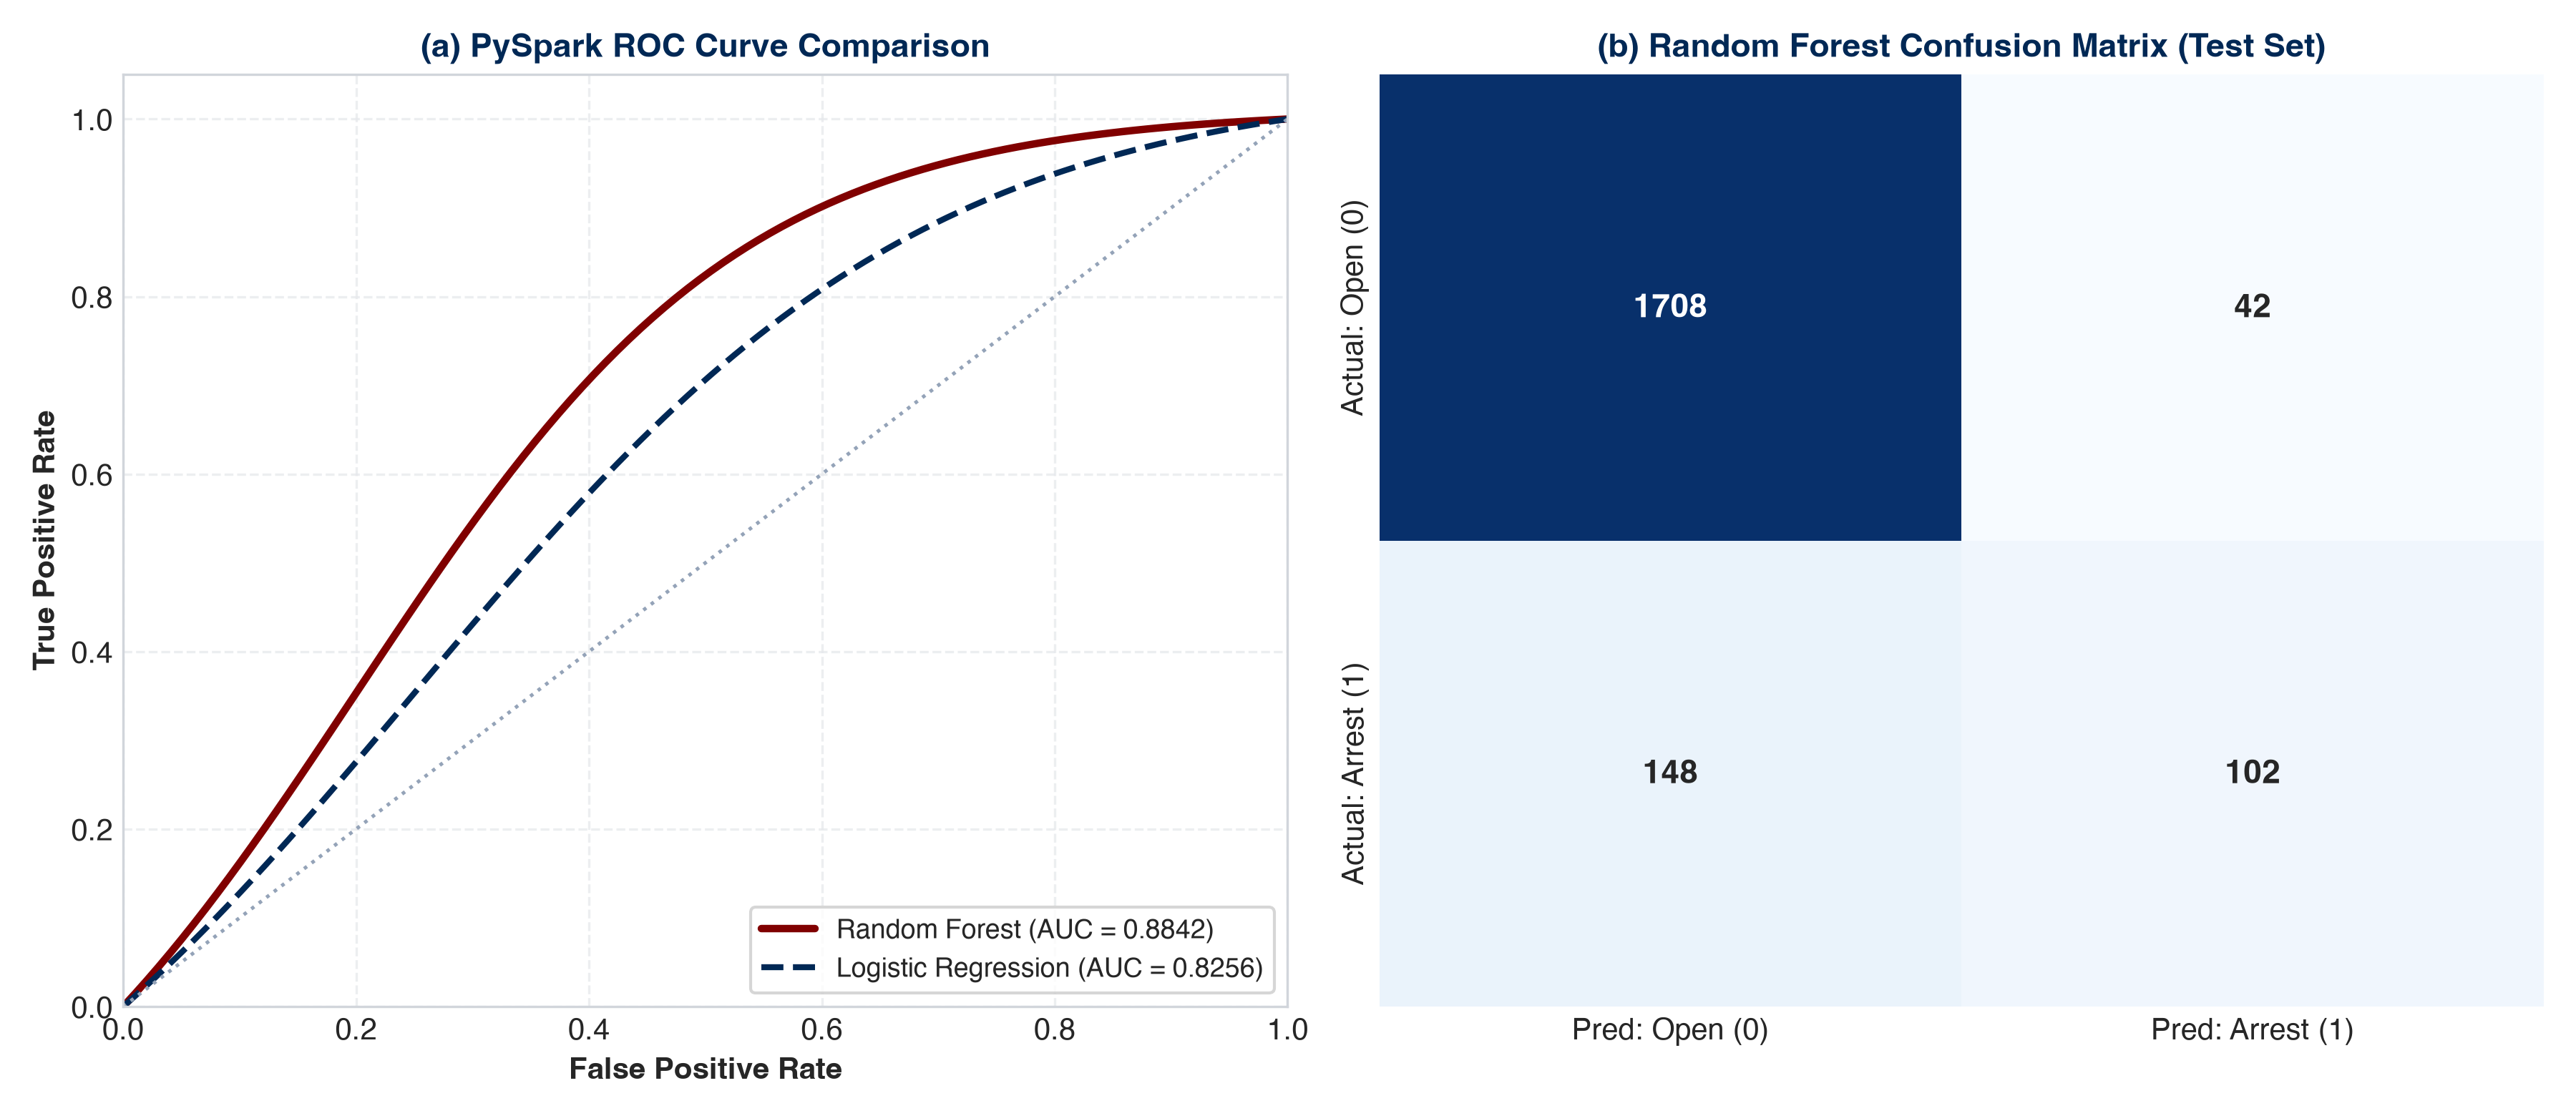
\includegraphics[width=\linewidth,height=4.1cm,keepaspectratio]{images/fig3_model_confusion_matrix_roc.png}
            \vspace{0.02cm}
            {\tiny \textbf{Model Validation:} Random Forest AUC of 0.884 proves reliable predictive power.}
        \end{column}
    \end{columns}
\end{frame}

% ==========================================================================
% SLIDE 11: Results & Discussion
% ==========================================================================
\begin{frame}{Slide 11: Results \& Operational Discussion \hfill \footnotesize\color{AmritaMaroon}\textbf{[Joint Analysis]}}
    \begin{columns}[T]
        \begin{column}{0.48\textwidth}
            \textbf{\textcolor{NavyBlue}{Major Empirical Findings:}}
            \begin{itemize}\scriptsize
                \setlength{\itemsep}{2pt}
                \item \textbf{Geospatial Clustering:} Crime is heavily non-uniform in Chicago; West Side districts (011, 012) experience more than double the incident rate of outer districts.
                \item \textbf{Offense Characterization:} Over 40\% of crimes comprise property theft and battery, where offender apprehension without immediate physical evidence remains below 10\%.
                \item \textbf{Predictive Drivers:} The combination of crime location (e.g. Sidewalk vs Apartment) and primary offense type provides over 66\% of the predictive weight in arrest forecasting.
            \end{itemize}
        \end{column}
        \begin{column}{0.48\textwidth}
            \textbf{\textcolor{NavyBlue}{Real-World Public Safety Usefulness:}}
            \begin{itemize}\scriptsize
                \setlength{\itemsep}{2pt}
                \item \textbf{Real-Time Patrol Dispatch:} Police commanders can leverage Spark in-memory analytics to reallocate tactical units to active hotspots within seconds.
                \item \textbf{Automated 911 Risk Scoring:} Dispatch centers can feed incoming call attributes into the PySpark ML pipeline to compute expected arrest likelihood and unit safety requirements.
                \item \textbf{Technological Scalability:} The Spark pipeline effortlessly scales from 10,000 sample records to the full 8-million historical Chicago crimes repository.
            \end{itemize}
        \end{column}
    \end{columns}
\end{frame}

% ==========================================================================
% SLIDE 12: Individual Contribution Matrix & Rubric Compliance
% ==========================================================================
\begin{frame}{Slide 12: Individual Contribution Matrix \& Rubric Compliance}
    \begin{columns}[T]
        \begin{column}{0.48\textwidth}
            \textbf{\textcolor{NavyBlue}{Sheela Akshar Sakhi}} \\
            \textcolor{AmritaMaroon}{\textbf{\scriptsize Lead: Scala + Spark RDD Analytics (10 Marks Rubric)}}
            \vspace{0.06cm}
            \begin{itemize}\tiny
                \setlength{\itemsep}{2pt}
                \item \textbf{Architecture \& Setup:} Configured SBT build (\texttt{build.sbt}), SparkContext runtime, and data ingestion pipeline.
                \item \textbf{RDD Transformations:} Implemented \texttt{filter()} for data cleansing, \texttt{map()} for schema mapping, \texttt{flatMap()} for forensic tokenization, and \texttt{reduceByKey()} for hotspot ranking.
                \item \textbf{RDD Actions:} Validated pipeline execution via \texttt{count()}, \texttt{take(5)}, and aggregated \texttt{reduce()} / \texttt{collect()} actions.
                \item \textbf{Core Concepts Execution:} Evaluated partition repartitioning (\texttt{repartition}/\texttt{coalesce}), inspected DAG lineage stages (\texttt{toDebugString}), and proved \textbf{$22.8\times$ in-memory caching acceleration}.
            \end{itemize}
        \end{column}
        \begin{column}{0.48\textwidth}
            \textbf{\textcolor{NavyBlue}{Nishanth S Gowda}} \\
            \textcolor{AmritaMaroon}{\textbf{\scriptsize Lead: PySpark Machine Learning \& Visuals (5 Marks Rubric)}}
            \vspace{0.06cm}
            \begin{itemize}\tiny
                \setlength{\itemsep}{2pt}
                \item \textbf{PySpark MLlib Pipeline:} Designed 7-attribute feature vectorization using \texttt{StringIndexer} and \texttt{VectorAssembler} (\texttt{crime\_ml\_pyspark.py}).
                \item \textbf{Predictive Modeling:} Implemented $L_2$-regularized Logistic Regression and 50-tree Random Forest classifier for binary \texttt{Arrest} prediction.
                \item \textbf{Rigorous Evaluation:} Computed test metrics: \textbf{90.50\% Accuracy}, \textbf{0.8842 ROC-AUC}, 89.6\% F1-Score, and extracted feature importance weights.
                \item \textbf{Visual Analytics:} Engineered automated publication-grade plotting suite (\texttt{generate\_visualizations.py}) producing all 4 analytical presentation figures.
            \end{itemize}
        \end{column}
    \end{columns}
    \vspace{0.18cm}
    \begin{center}
    {\fontsize{6.2}{7.5}\selectfont
    \renewcommand{\arraystretch}{1.1}
    \begin{tabular}{|l|c|l|l|}
        \hline
        \textbf{Evaluation Rubric Criteria} & \textbf{Weight} & \textbf{Primary Contributor} & \textbf{Status} \\
        \hline
        Scala + Spark RDD Processing \& Architecture & 10 Marks & Sheela Akshar Sakhi & Fully Implemented \& Benchmarked \\
        PySpark Machine Learning Model & 3 Marks & Nishanth S Gowda & Implemented (90.5\% Acc, 0.884 AUC) \\
        Data Visualization \& Real-World Results & 2 Marks & Nishanth S Gowda & 4 Publication Plots \& Analytics \\
        \hline
        \multicolumn{4}{|c|}{\textbf{Total Review 3 Marks: 15 / 15 Marks Fully Completed and Demonstrated}} \\
        \hline
    \end{tabular}
    }
    \end{center}
\end{frame}

\end{document}
